% Drawing 144/05-6 -- folder 144, batch 05, archive page 96 (PDF page 97).
% Transcription: en marge, un hexagone régulier inscrit dans un cercle, de sommets $A$, $C'$, $B$, $A'$, $C$, $B'$ ; les deux triangles $ABC$ et $A'B'C'$ y sont tracés.
% Kind: regular hexagon in a circle with triangles ABC, A'B'C'. Method 2 (schematic redraw from the facsimile). Status: ok.
% Notes: Pencil; the vertices in the cyclic order A, B', C, A', B, C' (clockwise from the top as drawn; the transcription lists them A, C', B, A', C, B' counter-clockwise, which is the same cycle).
% Coordinates: 1 unit = 1 mm = 1/100 of the crop width (bbox in page fractions: [0.11, 0.71, 0.3, 0.84]).
% Redrawn by Claude (claude-opus-5-5), issue #73, 2026-11-07; not checked by a human; not compiled (no TeX in the session).
% Rights: reproduces part of the work -- behind RENDER_TRANSCRIPTS, never published by itself.
\documentclass[tikz,border=3pt]{standalone}
\usepackage{amsmath,amssymb}
\usetikzlibrary{patterns,arrows.meta}
\tikzset{pencil/.style={black!45}, struck/.style={black!35}, mark/.style={circle,draw,inner sep=1.3pt}, pt/.style={circle,fill,inner sep=0.9pt}, opt/.style={circle,draw,fill=white,inner sep=1.1pt}}
\begin{document}
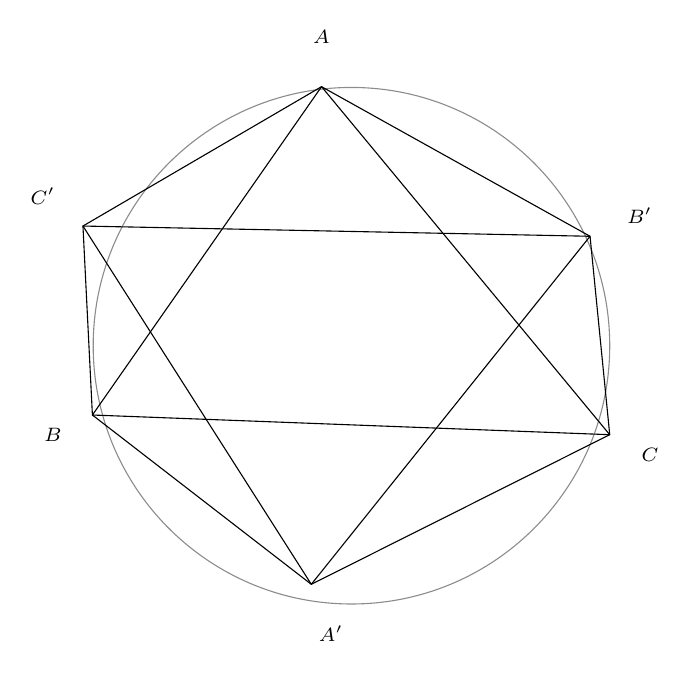
\begin{tikzpicture}[x=1mm,y=1mm,line cap=round,line join=round,font=\scriptsize]
\draw[pencil] (53.3,-49.3) circle[radius=32.8];
\draw (49.5,-16.4) -- (83.6,-35.4) -- (86.1,-60.6) -- (48.2,-79.6) -- (20.4,-58.1) -- (19.2,-34.1) -- cycle;
\draw (49.5,-16.4) -- (86.1,-60.6) -- (20.4,-58.1) -- cycle;
\draw (83.6,-35.4) -- (48.2,-79.6) -- (19.2,-34.1) -- cycle;
\node[inner sep=1pt] at (49.5,-10.1) {\scriptsize $A$};
\node[inner sep=1pt] at (89.9,-32.8) {\scriptsize $B'$};
\node[inner sep=1pt] at (91.2,-63.2) {\scriptsize $C$};
\node[inner sep=1pt] at (50.7,-85.9) {\scriptsize $A'$};
\node[inner sep=1pt] at (15.4,-60.6) {\scriptsize $B$};
\node[inner sep=1pt] at (14.1,-30.3) {\scriptsize $C'$};
\end{tikzpicture}
\end{document}
